%%Relayattack part in the article on PKE

\subsection{Relayattacks}
\subsubsection*{Idea}
%Describe attack idea
	As described before relay attacks base on the problem of localization in
	wireless networks.
	Attacking a passive Key-less entry system,
	the attacker relays the probing signal emitted from the car to the victims
	customer identification device (CID).
	The CID the emits a signal that opens the doors of the vehicle.
	Now the attacker can enter the car and again relay the signals emitted by the
	car so that he can ignite the engine.
	
	This method has been practically tested on different PKE systems by %TODO \citea{} %DER Artikel
	The authors showed that it is an eqsy and feasible attack.
	It also does not require very specialized hard- or software and
	the required components can be easily aquired with a relatively small budget.
	The relay attack is transarparent to any higher layer cryptography,	%transport layer?
	and so can easily circumvent the security systems of most PKE systems.

\subsubsection*{Variants}
	There are some variants in attacking PKE systems.
	Altough the attack could be in principle be carried out by one attacker alone,
	the literature usually asumes at leats two attackers.

%two thieves
	\label{par:twoThieves}
	Having two attackers performing a relay attack,
	the roles are split.
	The first thieves will try to get close to the victim and place
	the sending device close to the victims CID.
	This could take place in a store,
	where it doesnt raise attention to the victim if the attacker
	is in range of the CID.
	The second thief will be near the car,
	probably parked on the stores own carlot,
	to capture its probing signals.

	Now the signals are relayed between the CID and the car,
	and the car might open and start,
	allowing the second thiee to drive away.

%three thieves
\subsubsection*{Material \& Methods}
	This Section refers to the publication of \citeauthor{relayAttacksFranc} from \citeyear{relayAttacksFranc}
	and the tested approaches by the authors.

	%describe methods hwo to relate the signals, cable and wireless and its implications
	%describe what materials where
%Over the Cable
	\begin{figure*}[htb]
		\begin{center}
			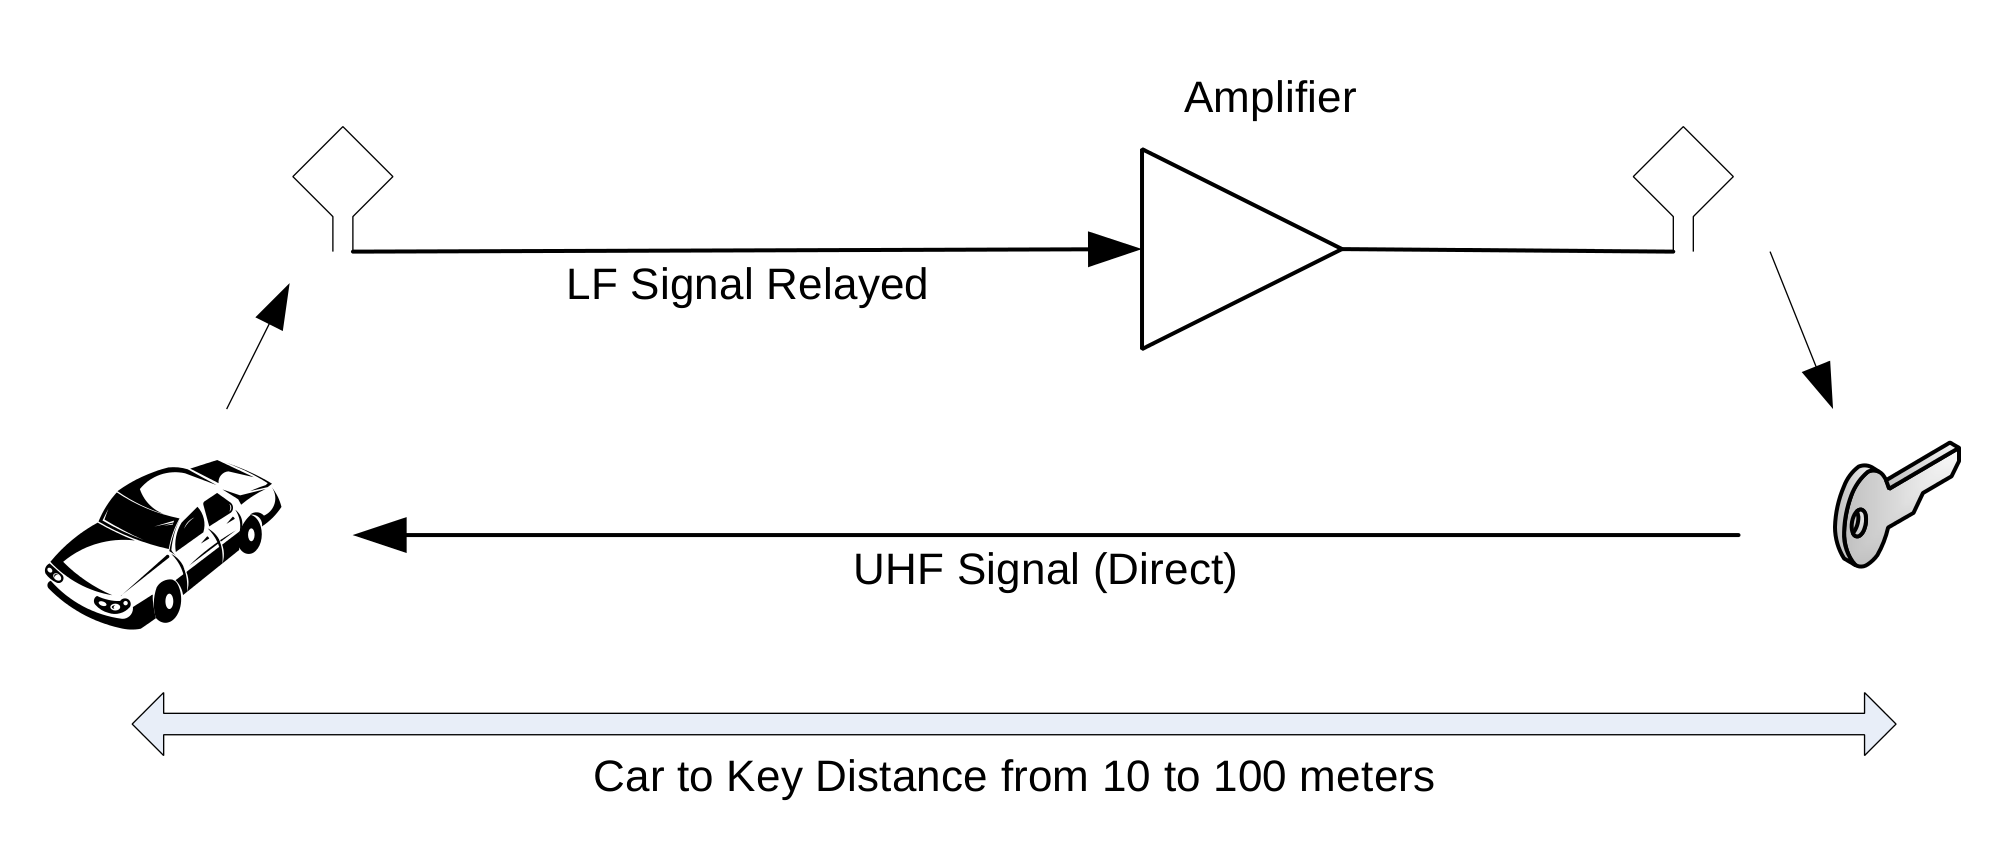
\includegraphics[width=\textwidth]{pictures/franc_relay_over_the_wire.png}
		\end{center}
		\caption{Relay wih antennas, cable and amplifiers \citep[p. 5]{relayAttacksFranc}.}
		\label{fig:relayOTC}
	\end{figure*}

	Relay  attacks on PKE systems can be carried out in different ways.
	In the most simple case,
	a cable is used to relay the transmitted LF signal from the car near the CID.
	An Amplifier might be needed to keep the signal stron enough.
	The keys UHF sender is strong enough so that the car will receive the send out signals.
	This case is shown in Figure %\ref{fig:relayByCalbe} %TODO create graphics
	Amplifiers might be nesscessary deping on the length of the cable,
	the quality of the antennas and the strength of the signal.

%Over the air
	\begin{figure*}[htb]
		\begin{center}
			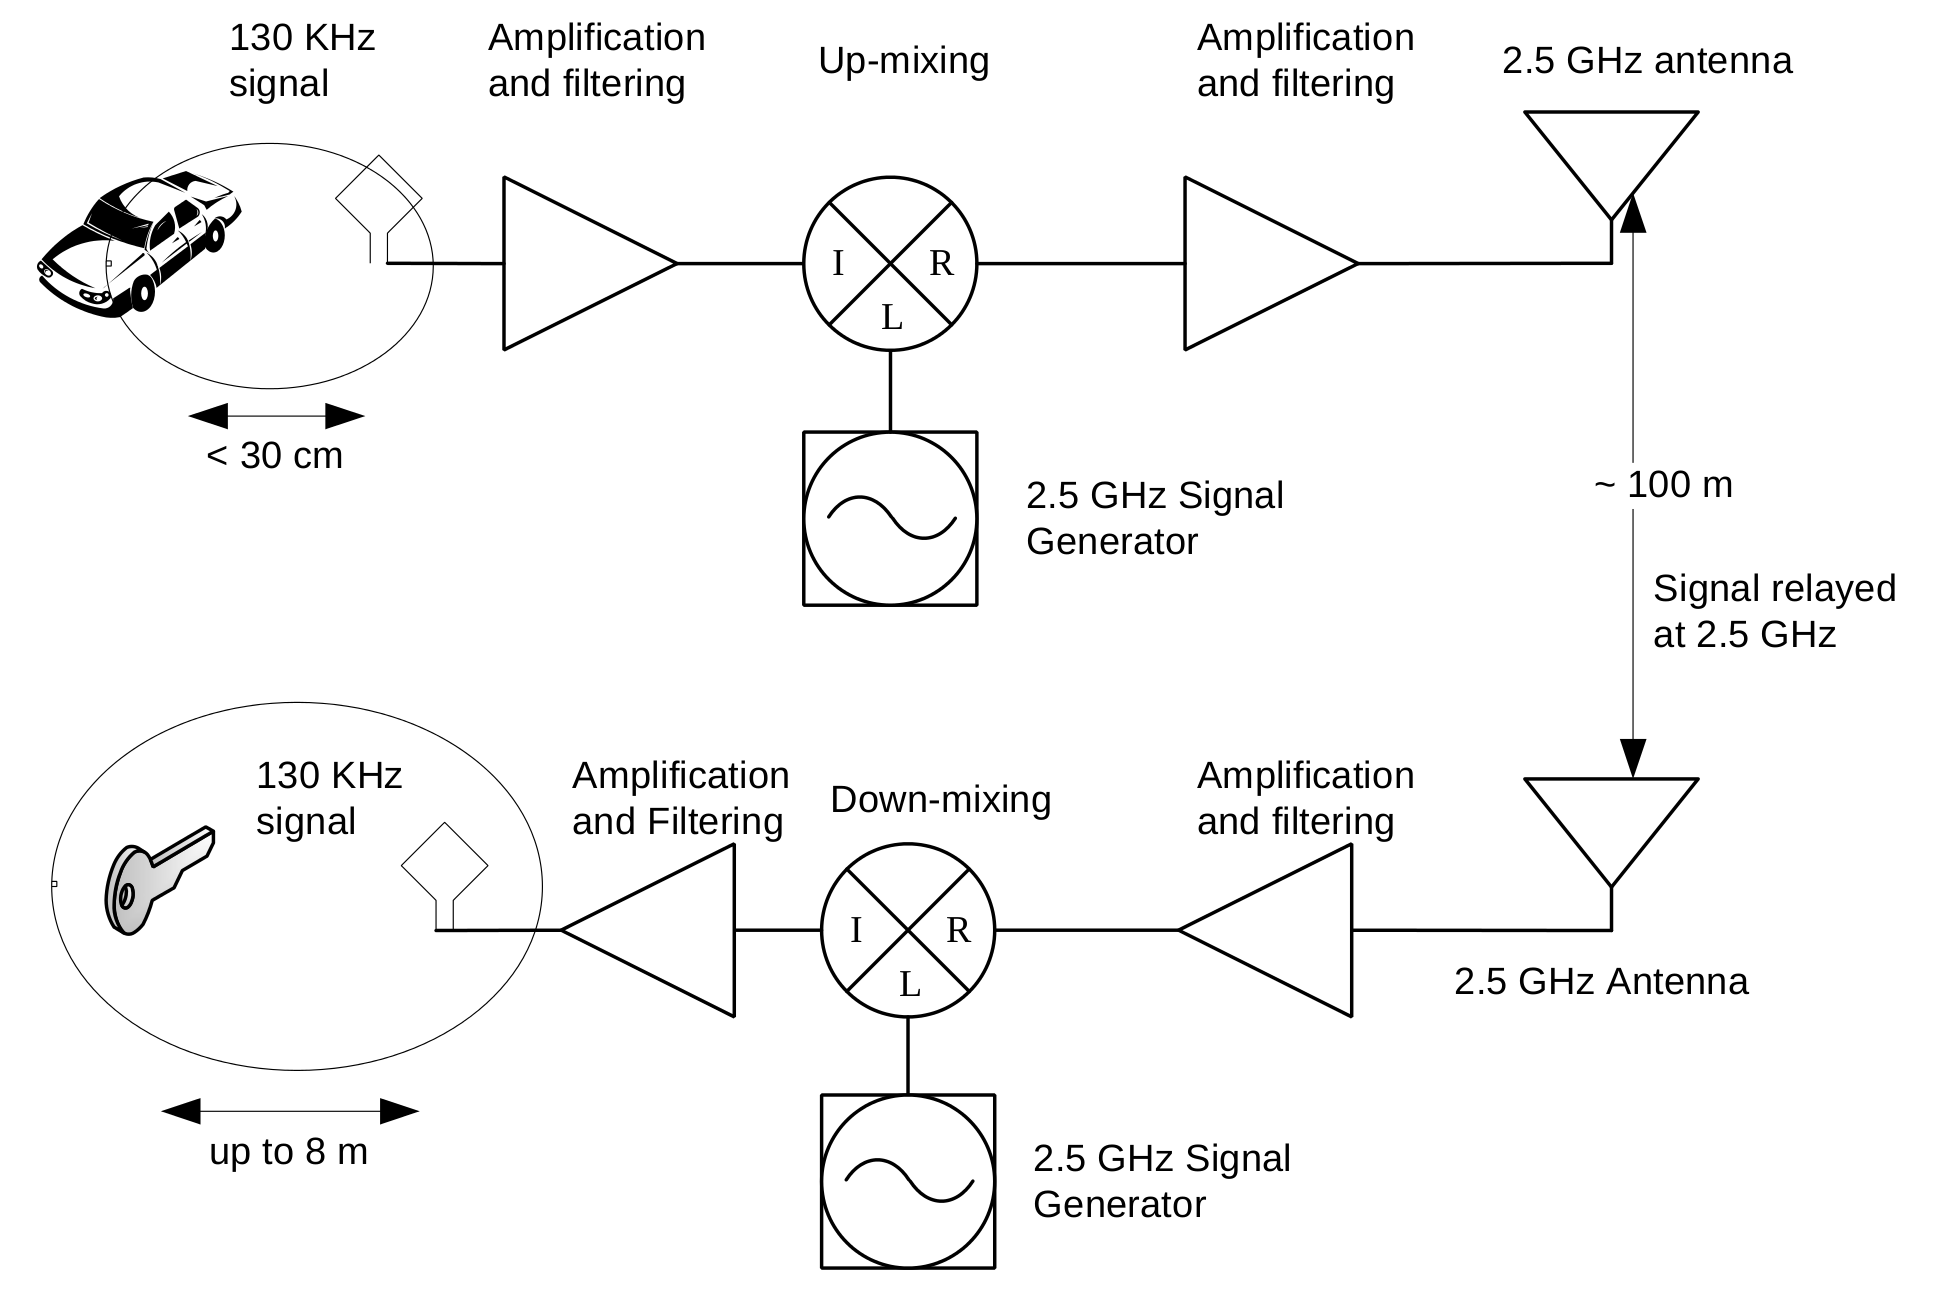
\includegraphics[width=\textwidth]{pictures/franc_relay_over_the_air.png}
		\end{center}
		\caption{Relay over-the-air with up- and downconversion and amplifiers \citep[p. 6]{relayAttacksFranc}.}
		\label{fig:relayOTA}
	\end{figure*}
	A cable is rather impractical to relay the signal.
	\citeauthor{relayAttacksFranc} used upconversion and downconversion to realy the signal.
	The 130 kHz signal transimetted by the car is amplified and upconverted to a 2.5 GHz signal.
	This signal is send out to a 2.5 GHz antenna and downmodulated to 130 KHz again.
	Amplifiers are used as required by signal strength and quality.
	The conversion steps are down analog,
	to ensure a fast conversion rate.
	Also this keeps the attack simple and inexpensive.
	Figure \ref{fig:relayOTA} show the layout of the Relay over-the-air attack.

%Cars
	\citeauthor{relayAttacksFranc} acqiured 10 distinct car models that have been build by 8 different manufacturers.
	The cars were from different types,
	there were \$sedans, \$SUVs, \$sportscars  and \$sedans.
	They also tested \$aftermarket PKE-systems.
	The authors tested the relay attack in \$different settings.

	Firstofall the authors tested the attack using a wired connection,
	to relay the CID and the vehicle.

	The authors also used a wireless aproach to establish a link between the CID and the vehicle.

\subsubsection*{Results}
	%results francillion et al. achieved with real world cars
	The Authors were able to succesfully carry the attack out to various number of cars.
	They aquired 10 different car models from 8 manufacturers.
	These models were tested if they were vulnerable against the two thieves attack as described in 
	Section \ref{par:twoThieves}.
	\citeauthor{relayAttacksFranc} were able to excite the CID from ranges up to 8 meters
	and therefore open the car altough the car was more than 50 meters away.

\subsection*{Implications}
	\label{sec:attackImplications}
	Gaining access to a vehicle as great implications for the overall security of a car.
	Stealing the car is the straightforward approach,
	but in combination with attacks on the cars internal electronic system,
	malvolent attacks on the vehicle and its passenger are possible.

	Modern vehicles are controlled by many small electronic computing units (ECU),
	whom are interconnected over a bus system.
	Prominent ECUs manage the engine, the breaks or the Electronic devices on the dasboard.
	The more security relevant ECUs are connected via a priviledged,
	high-speed bus,
	where less important ones use a seperate lower-speed bus.
	These bus-systems should be strictly seperate as specified in the standard. %TODO cite standard for OMB bla
	Seperating the communication of the brakes and windscreenwipers,
	shall ensure that the integral systems keep working,
	when it is acceptable that less important ones can fail.

	However the article form \citeauthor{expModernAuto} %TODO CITE!
	shows that these security features and the standards were not implemented as intended.
	%TODO \citea{}
	point out what can be done if access to the to the electronic bus system can be achieved.
	They were able to cut the engine and the engage single brakes,
	even while driving.
	%TODO \citea{}
	point out that it is not possible to traceback certain attacks.	%verify that

	%what harm can occur from gaining unnotices acces to the vehicle
